\subsection{Strom-Spannungs-Kennlinien}

% FEHLT:
% - Formatierung überprüfen ([h],... bei figures und Paragaphen einrücen überpr.)

Die Strom-Spannungs-Kennlinien des Photowiderstandes werden für verschiedene Wellenlängen aufgenommen. Dafür wird zunächst der Versuchsaufbau eingestellt. Der Photowiderstand wird horizontal und vertikal justiert, dann wird die Linse auf der Versuchsschiene bewegt, bis der gemessene Strom bei konstanter Spannung maximal ist. Diese Einstellungen werden im gesamten Versuchsverlauf nicht verändert. \\
Für Aufgabe 1 wird zusätzlich noch ein Farbfilter verwendet, der nur eine Wellenlänge durchlässt. Verwendet werden die Wellenlängen 647nm und 549nm. Zusätzlich wird das Licht im Versuchsraum ausgeschaltet, um Störeffekte zu minimieren. \\
\\
Die an dem Photowiderstand angelegte Spannung wird direkt an einem Computer mittels LabView eingestellt. Die gemessene Stromstärke wird dort auch angezeigt. So werden bei obigen Wellenlängen und bei abgedunkeltem Photowiderstand insgesamt drei Strom-Spannungskennlinien von 1V bis 10V in 1V-Schritten aufgenommen. \\
Abb. 4.1 zeigt die gemessenen Datenpunkte und je einen linearen Fit. Die Geraden folgen der Gleichung $I = m \cdot U + c$ mit den in Abb. 4.2 angegebenen Parametern. \\
Sowohl Spannung als auch Stromstärke sind fehlerbehaftet, jedoch ist uns auf Grund des Versuchsaufbaus nicht möglich diese genau anzugeben. Eine grobe Schätzung basierend auf dem Schwanken der Anzeige ist es für die Stromstärke einen statistischen Fehler von 0.01 mA und für die Spannung von 0.1 V anzunehmen. Bei der Berechnung der Regressionsgeraden werden diese verwendet.

\begin{figure}
\label{A1_reg}
\centering
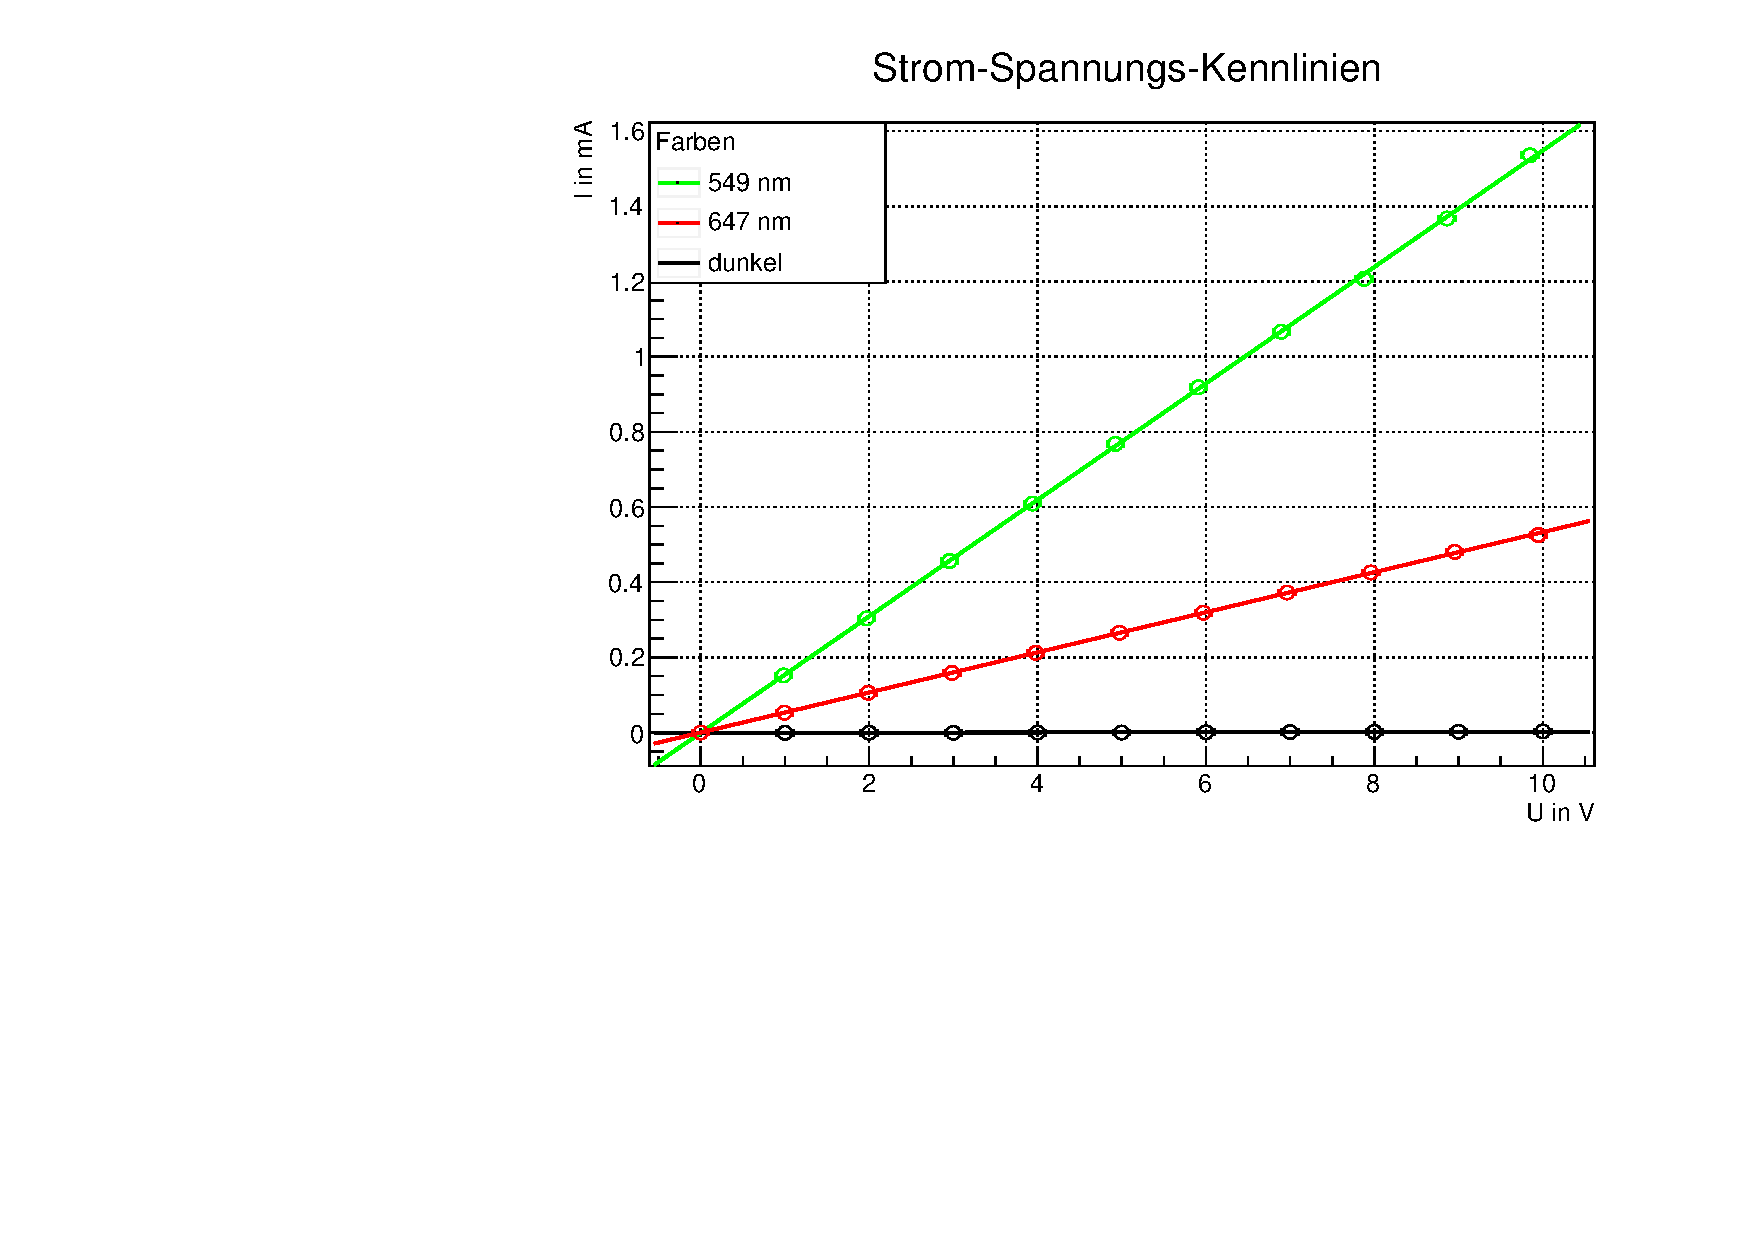
\includegraphics[scale=0.5]{Messdaten/A1.pdf}
\caption{Strom-Spannungskennlinien des Photowiderstandes bei den Wellenlängen 549nm, 647nm sowie ohne Lichteinstrahlung. Ein linearer Zusammenhang wird erkannt und eine lineare Regression wurde durchgeführt. Die Steigung ist offensichtlich abhängig von der Wellenlänge.}
\end{figure}

\begin{figure}
\label{A1_param}
\centering
\caption{Parameter der drei Regressionsgeraden}
\vspace{0.4cm}
\begin{tabular}{lccc}
& dunkel & 647 nm & 549 nm \\ 
\hline
\hline
$\mathrm{m} \ /\ \frac{mA}{V} $& $(3.40 \pm 9.53) \cdot 10^{-4}$ & $(5.33 \pm 0.11) \cdot 10^{-2}$ & $(1.55 \pm 0.02) \cdot 10^{-1}$\\
$c\ /mA$ & $(-1.03 \pm 5.64) \cdot 10^{-3}$ & $(0.18 \pm 6.39) \cdot 10^{-4} $ & $(-0.06 \pm 1.04) \cdot 10^{-2}$ \\
\end{tabular}
\end{figure}


Die Messung liefert gemäß dem Ohm'schen Gesetz einen linearen Zusammenhang von Strom und Spannung für eine konstante Wellenlänge. Die Steigung und damit der Widerstand sind abhängig von der Wellenlänge des eingestrahlten Lichtes. Ohne eingestrahltes Licht ist die Steigung nahezu 0 und somit der Widerstand praktisch unendlich. Mit sinkener Wellenlänge und damit steigender Energie des eingestrahlten Lichtes sinkt der Widerstand. \\
Das qualitative Ergebnis dieser Messungen deckt sich mit unseren Erwartungen. Ohne Lichteinstrahlung sind kaum Elektronen im Leitungsband des Photowiderstandes, lediglich durch das thermische Gleichgewicht bedingt. Steigt die Energie der Photonen, so können Elektronen aus dem Valenzband die Bandlücke überqueren und ins Leitungsband gelangen. Bei höherer Energie steigt die Anzahl der Elektronen, die so angeregt werden können und damit die Leitfähigkeit. Außerdem stellt sich ein Gleichgewicht zwischen Rekombination und Anregung ein, wodurch die Anzahl der freien Ladungsträger und damit auch die Leitfähigkeit konstant ist. \\
In Aufgabe 3 wird die Leitfähigkeit in Abhängigkeit der Wellenlänge genauer untersucht. Unter anderem steigt die Leitfähigkeit nicht zwangsläufig mit zunehmender Energie der Photonen. \\

\subsection{Intensität}

\subsection{Frequenz}

\subsection{Lebensdauer}
% FEHLT:
% - Formatierung ([c],[h],... bei figures, Paragraphen eingerückt?)
% - Abb. Nummerierung überprüfen

Es wird nun die Lebensdauer der Elektronen bestimmt, indem eine sinusförmig modulierte Lichtquelle verwendet wird. \\
Dazu wird die Halogenlampe ausgeschalten und eine blaue Leuchtdiode mit modulierter Instensität verwendet. Die Frequenz der Modulation kann in LabView eingestellt werden, sowie die Amplitude des variierenden Photostroms und die dazugehörige Phasenverschiebung abgelesen werden. Die eingestellt Frequenz wird mit einer weiteren Silizium-Photodiode und einem Oszilloskop nachgemessen und an einen Lock-In-Verstärker angeschlossen. Dieser misst dann über einen zu dem Photowiderstand in Serie geschalteten Widerstand den Photostrom. \\
\\
Wie im letzten Abschnitt der Vorbereitung erwähnt werden nun die Amplitude und die Frequenz in einem doppelt logarithmischen Graphen dargestellt und der Anfangs- bzw. Endbereich zur Berechnung von Regressionsgeraden verwendet. \\
Abb. 4.3 zeigt die Messwerte und diese beiden Geraden graphisch dargestellt. Zur Berechnung der horizontalen Gerade wurden die ersten vier Messpunkte verwendet, für die zweite Gerade die letzten sieben. 
Die beiden Geraden folgen der Gleichung $\mathrm{log} (A / \mu A) = m \cdot log(\omega / Hz) + c$ mit den in Abb. 4.4 angegebenen Parametern. \\

\begin{figure}
\label{A4_reg}
\centering
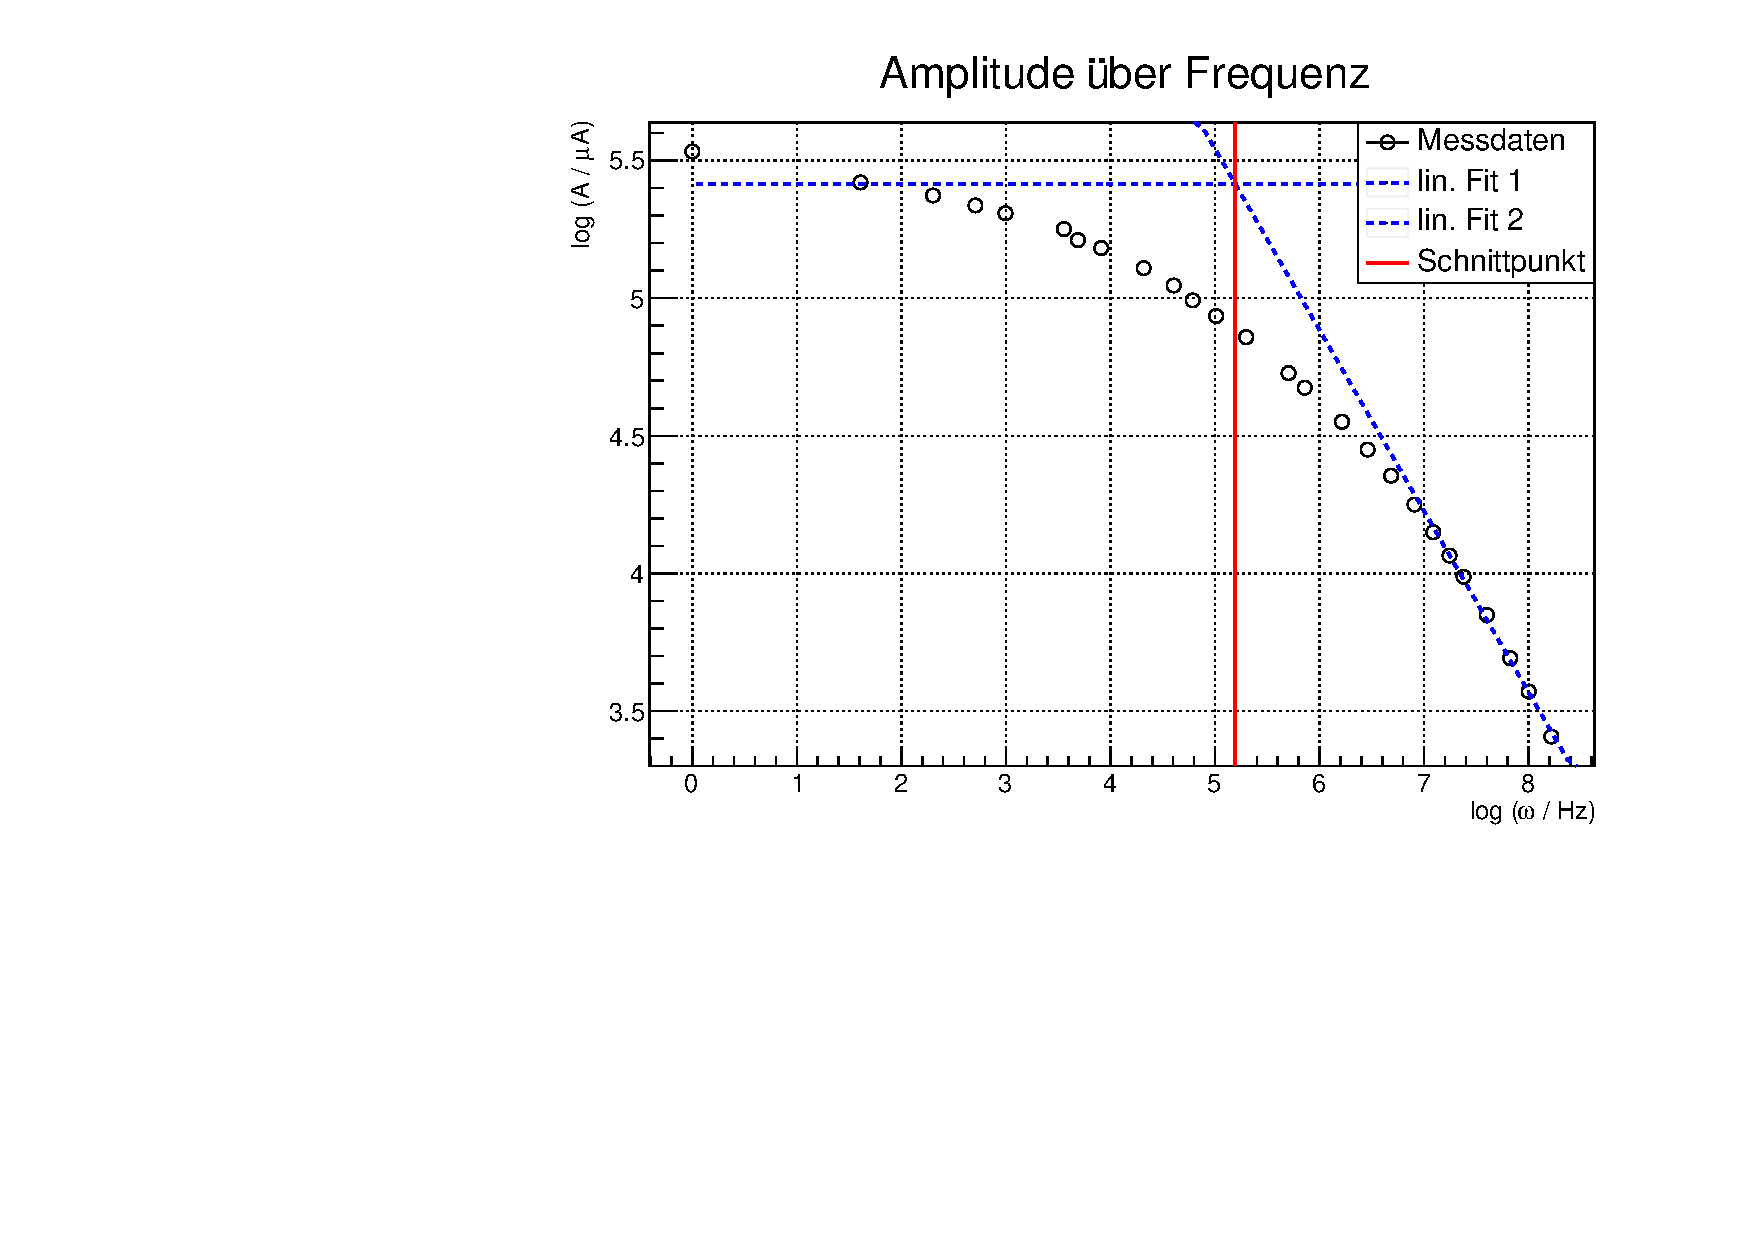
\includegraphics[scale=0.5]{Messdaten/A4_2fits.pdf}
\caption{Logarithmus der Photostromamplitude über dem Logarithmus der Frequenz. Die beiden Endbereiche wurden linear gefittet. Der Schnittpunkt der beiden Geraden ist laut Vorbereitung bei $\omega \cdot \tau = 1$, woraus die mittlere Lebensdauer der Elektronen folgt.}
\end{figure}


\begin{figure}
\label{A4_param}
\caption{Parameter der Regressionsgeraden in den beiden Frequenzbereichen}
\vspace{0.4cm}
\begin{tabular}{lcc}
& niedrige Frequenzen & hohe Frequenzen \\ 
\hline
\hline
m & 0 & $-0.658 \pm 0.015$\\
c & $5.416 \pm 0.043$ & $8.833 \pm 0.116$ \\
\end{tabular}
\end{figure}

Der Schnittpunkt liegt bei 
$$\log(\omega _{intersect.} / Hz) = 5.193 \pm 0.918$$
woraus nach Vorbereitung folgt:
$$\omega = (180.009 \pm 165.009) Hz $$
$$\tau = \frac{1}{\omega _{intersect.}} = (5.556 \pm 5.100) ms$$

Auf den ersten Blick fällt die sehr hohe Messungenauigkeit der mittleren Lebensdauer $\tau$ auf. Der Grund dafür liegt darin, dass schon die kleinen Unsicherheiten der Regressionsgeraden durch Umkehren des Logarithmus große Auswirkungen haben. \\
Vernachlässigt wurden dabei noch Unsicherheiten der aufgenommenen Messwerte auf Grund des Messapparates. Außerdem ist die Wahl der verwendeten Punkte in Abb. 4.3 nicht eindeutig, wodurch sich das Ergebnis ändern könnte.\\
Alledem ist die Größenordnung gut erkennbar und liegt im einstelligen ms-Bereich.  

